% BE�LL�T�SOK - JOBB NEM V�LTOZTATNI

\documentclass[final]{ubb_dolgozat}
\usepackage{definitions}
\usepackage{pdfpages}
\usepackage{listings}

\newcommand{\pdf}[1]{pythonCodes/#1.pdf}
%%


% milyen nyelveken akarunk forr�sk�dot megjelen�teni
\lstloadlanguages{C, C++, Python}

% ezt be lehet tenni MINDEGYIK megjelen�tend� k�d el�.
\lstset{language=Python}


%% MELYIK �VBEN ADJUK LE
\submityear{%
2015
}
%% MELYIK H�NAPBAN ADJUK LE
\submitmonthHU{%
J�lius
}
\submitmonthRO{%
Iulie
}
\submitmonthEN{%
July
}

\titleHU{%
Forgalmi t�bl�k felismer�se
}
\titleEN{%
Road sign recognition
}

\titleRO{%
Recunoa\c{s}terea semnelor de circula\c{t}ie
}

\author{%
Szabo �gnes-Ter�z
}

%%
\tutorHU{%
Csat� Lehel\\
 {\large Babe\c{s}--Bolyai Tudom�nyegyetem,\\
 Matematika �s Informatika Kar}
}

%%
\tutorRO{%
Csat� Lehel\\
 {\large Universitatea Babe\c{s}--Bolyai,\\
 Facultatea de Matematic\u{a} \c{s}i Informatic\u{a} }%
}
%%
\tutorEN{%
Csat� Lehel
 {\large Babe\c{s}--Bolyai University,\\
 Faculty of Mathematics and Informatics}
}


%\includeonly{bevezet}


\begin{document}

%% ABSTRAKT
\begin{abstractEN} % ANGOL V�LTOZAT

\vfill
I work on a system which as an input gets a sound file, proccesses it, analyzes it, and as an output generates a sheet music, which contains the detected music notes from the sound file.


This work is the result of my own activity. I have neither given nor received unauthorized assistance on this work.

\vfill

\end{abstractEN}


% ez a c�moldal r�sze
\maketitle
%% 

% a dolgozat tartalomjegyz�ke -- ez automatikusan gener�l�dik a STRUKT�RA alapj�n.
{ \baselineskip 1ex
  \parskip 1ex
  \tableofcontents
}


%%%%%%%%%%%%%%%%%%%%%%%%%%%%%%%%%%%%%%%%%%%%%%%%%%%%%%%%%%%
%%%%%%%%%%         a dolgozat tartalma         %%%%%%%%%%%%



% a bevezet� fejezet FILE-ja.
%!TEX root = dolgozat.tex
%%%%%%%%%%%%%%%%%%%%%%%%%%%%%%%%%%%%%%%%%%%%%%%%%%%%%%%%%%%%%%%%%%%%%%%
\chapter{Bevezető}\label{ch:INTRO}
%%%%%%%%%%%%%%%%%%%%%%%%%%%%%%%%%%%%%%%%%%%%%%%%%%%%%%%%%%%%%%%%%%%%%%%

\section{A dolgozat célja}\label{sec:INTRO:goal}
Számos olyan rendszer létezik ami megtalál és felismer forgalmi táblákat valós környezetből vett képeken, de a robusztus és költséghatékony megoldás a mai napig aktív kutatási téma. Mivel több különböző típusú forgalmi tábla létezik és ezek között sok a hasonlóság, a megkülönböztetésük a mai napig kihívásnak bizonyul. A táblák felismerhetőségét befolyásolja több tényező, mint a fényerősség, árnyékolás, parciális fedés és egyéb akadályok.

Egyes autóvezetők számára nehézséget jelenthet a figyelmük megosztása, ami bizonytalansághoz, balesethez vezethet. Ha rendelkezésükre állna egy rendszer, ami képes figyelmeztetni őket a forgalmi táblákról és az általuk megszabott korlátról vagy információról, magabiztosabbá válhatnának.

A célom egy gyors, hatékony és megbízható rendszer készítése forgalmi táblák felismerésére valós környezetben készített képekről.

\section{Megvalósítás}\label{sec:INTRO:implement}

A rendszer először előfeldolgozást végez a képeken. Mivel a tesztadatok nem azonos méretűek, átméretezi őket, majd szín szerinti szűrést végez, hogy egyszerűsítse a feldolgozandó adatokat. Ezt követően neurális háló segítségével elkezdődik a tanulási folyamat. Miután a rendszer megtanulta a különböző osztályok jellemzőit, a rendszer használható forgalmi táblák felismerésére tetszőlegesen kiválasztott képeken.

A felhasználó által kiválasztott képen elsősorban meg kell találni a forgalmi tábla helyét. Ennek érdekében a képet kisebb darabokra vágja és ezeken is végrehajtja a fentebb említett előfeldolgozást. Az így kapott képeken próbálja azonosítani a forgalmi táblákat.

Mivel a forgalmi táblák idővel változhatnak, lényeges szempont, hogy a tervezett rendszer könnyen alkalmazkodjon a változásokhoz, anélkül, hogy nagymértékben módosítani kelljen azt. A neurális hálók tökéletesek erre a feladatra, hiszen, ha az adatok változnak is, elég a tanulási folyamatot megismételni; nincs szükség a kód módosítására \cite{8}.
%!TEX root = dolgozat.tex
%%%%%%%%%%%%%%%%%%%%%%%%%%%%%%%%%%%%%%%%%%%%%%%%%%%%%%%%%%%%%%%%%%%%%%%
\chapter{Forgalmi táblák}\label{ch:SIGNS}
%%%%%%%%%%%%%%%%%%%%%%%%%%%%%%%%%%%%%%%%%%%%%%%%%%%%%%%%%%%%%%%%%%%%%%%

\section{Mik a forgalmi táblák?}\label{sec:SIGNS:whatAreThey}

A forgalmi táblák a forgalom irányításáért felelősek; figyelmeztetik, irányítják és informálják a gépkocsivezetőket. Három fő típusú forgalmi tábla van és mindegyik különböző formával rendelkezik:
\begin{compactenum}
	\item utasító táblák (kör)
	\item figyelmeztető táblák (háromszög)
	\item informáló táblák (téglalap)
\end{compactenum}

Ez alól kivétel a STOP tábla, ami nyolcszög alakú.

További információval szolgál a forgalmi tábláról a színe. A forgalmi táblák figyelemfelkeltőek kell legyenek, ennek megfelelően alkalmazzák a színeket is. A megjelenő színek: piros, fehér, fekete, sárga és kék \cite{8}.

A forgalmi táblák többsége két részből tevődik össze: egy külső telített sáv és egy belső szimbólum vagy szám. A belső szimbólum általában fekete. 


\section{Adathalmaz}\label{sec:SIGNS:dataSet}

Az adathalmazhoz egy forgalmi táblák felismerésére kitűzött németországi verseny adatait használtam fel \cite{9}.

\subsection{Tanulási adatok}

Az adathalmaz 1213 tanulási adatot tartalmaz. A képek mérete 16x16 pixeltől 128x128 pixelig változik, különböző szemszögből és változatos fényhatások mellett. A képek 43 kategóriába vannak sorolva, a tartalmazott forgalmi tábla alapján.

Habár nagy mennyiségű tanulási adat áll rendelkezésre, ezek nincsenek egyenlően elosztva az osztályok között. Ez megnehezíti a tanulást a neurális háló számára. Azok az osztályok amelyekben kevés tanulási adat van, kevésbé vannak befolyással a neurális háló kimenetére. 

A \ref{fig:trainingImage} ábrán látható példa négy tanítási adatra. Az első három képen levő táblák könnyedén felismerhetőek, míg a az utolsó tábla nehezen azonosítható. Nehéz megmondani, hogy 30-as, 70-es vagy 80-as sebességkorlát. Az adathalmazban kis számban ugyan, de előfordulnak ehhez hasonló táblák. Ezek megnehezítik a tanulási folyamatot.

\begin{figure}[h]
\centering
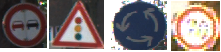
\includegraphics[scale=2]{images/train}
\caption{Példa tanulási adatokra}
\small forrás:\url{http://benchmark.ini.rub.de/?section=gtsdb&subsection=dataset}


\label{fig:trainingImage}
\end{figure}

\subsection{Tesztelési adatok}

900 teszt adat állt a rendelkezésemre, amiken nullától hatig akárhány forgalmi tábla megjelenhetett. Ezek jóval nagyobb méretű képek a tanításra szánt képeknél, 1360x800 pixel nagyságúak. A \ref{fig:testImage} ábrán látható egy példa ilyen képre. Ezen a képen két forgalmi tábla található.

\begin{figure}[h]
\centering

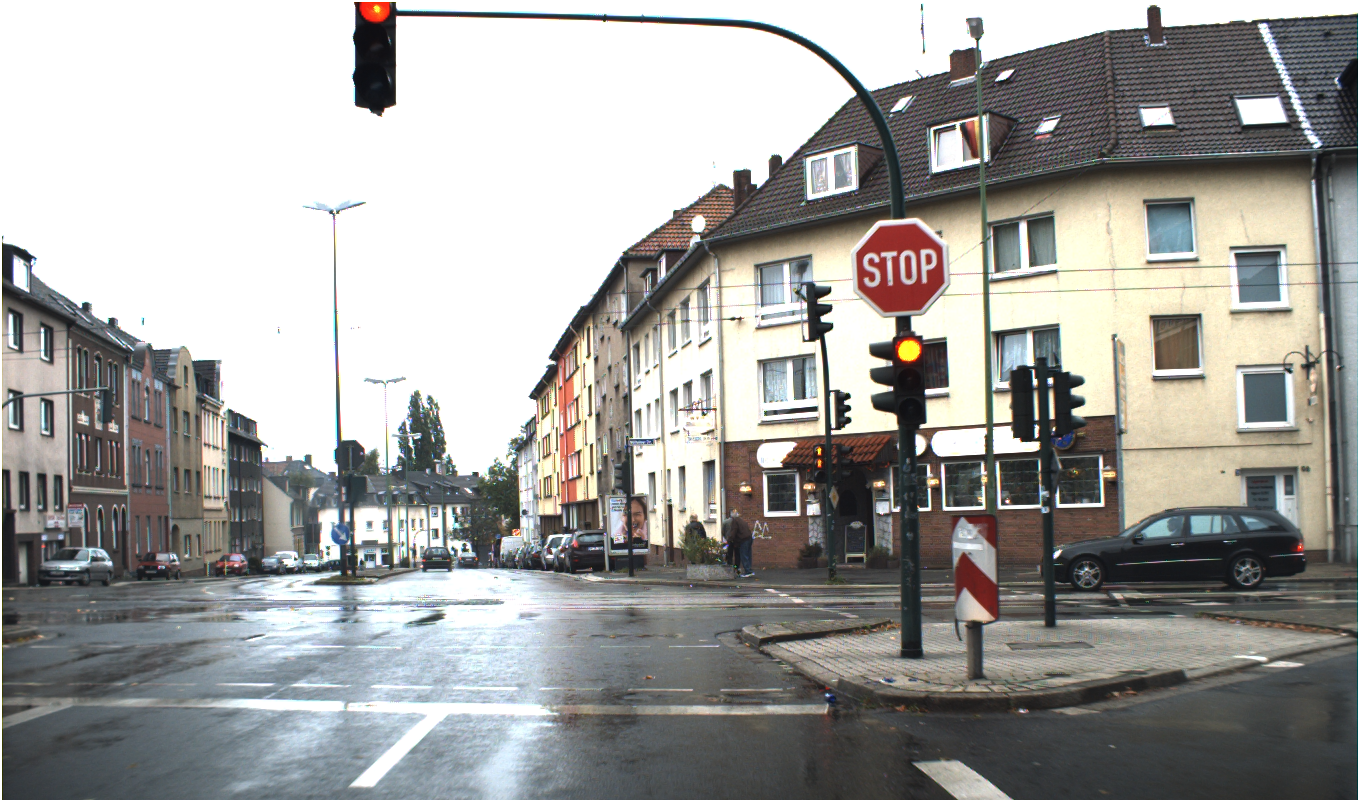
\includegraphics[scale=0.4]{testImage}
\caption{Példa teszt adatra}
\small forrás:\url{http://benchmark.ini.rub.de/?section=gtsdb&subsection=dataset}

\label{fig:testImage}
\end{figure}


%!TEX root = dolgozat.tex
%%%%%%%%%%%%%%%%%%%%%%%%%%%%%%%%%%%%%%%%%%%%%%%%%%%%%%%%%%%%%%%%%%%%%%%
\chapter{Darabolás}\label{ch:SEGMENT}
%%%%%%%%%%%%%%%%%%%%%%%%%%%%%%%%%%%%%%%%%%%%%%%%%%%%%%%%%%%%%%%%%%%%%%%

Annak érdekében, hogy megtaláljunk egy forgalmi táblát egy képen, szegmentációt alkalmaztam. A szegmentáció az a folyamat, amikor kisebb képeket vágunk ki egy nagyobb képből \cite{7}.

Több különböző módszer létezik a szegmentálás végrehajtására. Az általam alkalmazott véletlenszerű kiválasztáson alapszik. Véletlenszerű téglalapokat generálok és vágom ezeket ki az eredeti képből.

Mivel a valós környezetből vett képek több forgalmi táblát is tartalmazhatnak, fontos hogy az egész képet bejárják ezek a darabok. Azáltal, hogy nagy számban generálok ilyen darabokat, biztosítom, hogy nagy valószínűséggel megtaláljam a képen levő forgalmi táblákat. A táblák mérete is változik attól függően, hogy milyen távolságra van a fényképezőtől, ezért arra is figyelnem kellett, hogy a kivágott darabok mérete széles tartományban mozogjon.

Azáltal, hogy véletlenszerűen választom ki a vizsgálandó részeket az eredeti képből, ezeknek nagy része olyan kép lesz, ami nem tartalmaz forgalmi táblát vagy csak részlegesen fogja azt tartalmazni. Ez az oka annak, hogy a neurális háló akkor is megfelelően kell osztályozza a táblát ha csak 70-80\% látszik belőle.


\begin{figure}[h]
\centering

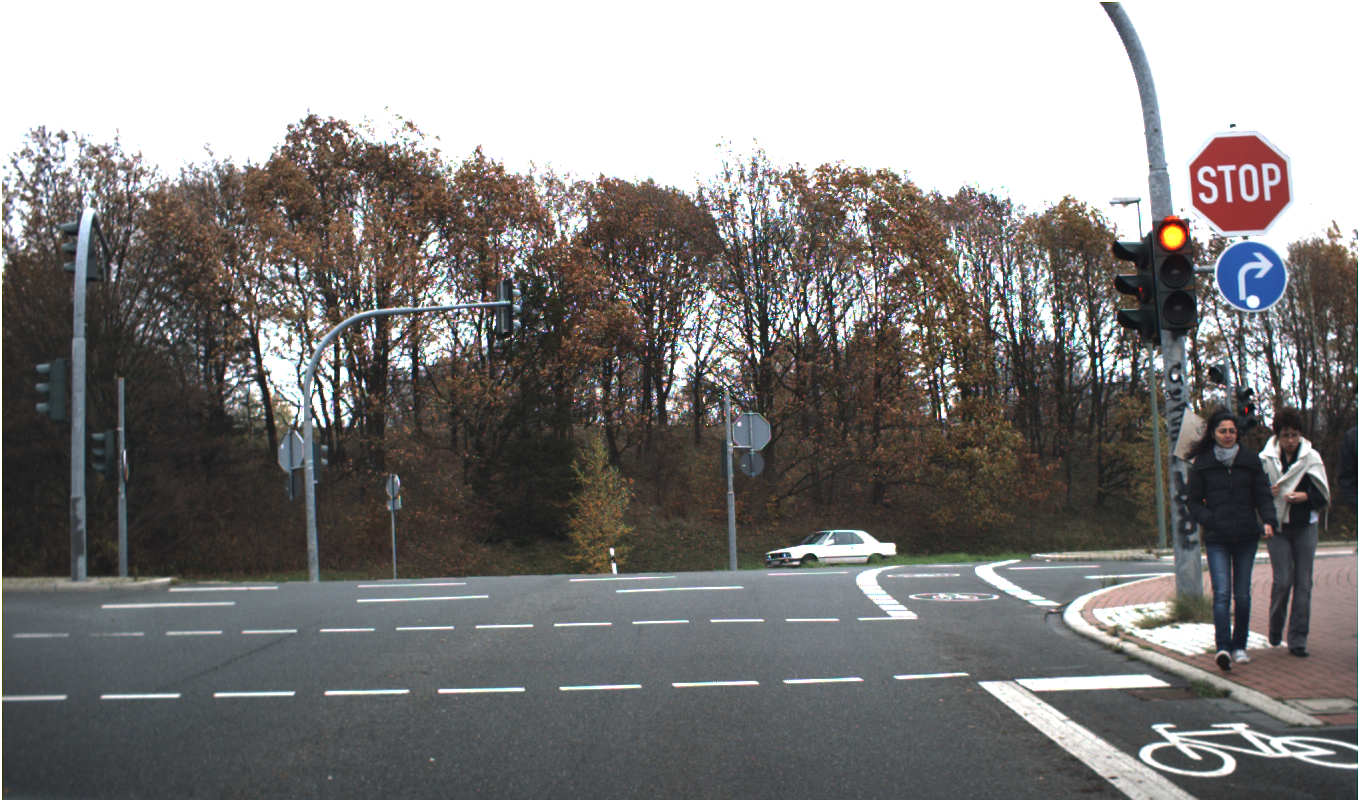
\includegraphics[scale=0.35]{images/testImage2}
\caption{Szegmentálás előtti kép}
\small forrás:\url{http://benchmark.ini.rub.de/?section=gtsdb&subsection=dataset}

\label{fig:testImage2}
\end{figure}

\begin{figure}[h]
\centering

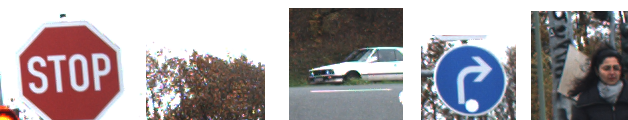
\includegraphics[scale=1]{images/segments}
\caption{Példa szegmentálás utáni képekre}
\small forrás:\url{http://benchmark.ini.rub.de/?section=gtsdb&subsection=dataset}

\label{fig:segments}
\end{figure}

A \ref{fig:testImage2} ábrán látható kép darabolásából nyert képekre látunk példákat a \ref{fig:segments} ábrán. Az így létrejött képek között megtalálható a két forgalmi tábla (első és negyedik kép) de ezeken kívül olyan darabok is létrejönnek, amik nem tartalmaznak forgalmi táblát. Azok a darabok amik nem tartalmaznak forgalmi táblát más információt tartalmaznak, mint például emberek, fák, járművek, esetleg hirdető táblák. 
%!TEX root = dolgozat.tex
%%%%%%%%%%%%%%%%%%%%%%%%%%%%%%%%%%%%%%%%%%%%%%%%%%%%%%%%%%%%%%%%%%%%%%%
\chapter{Preprocessing images}\label{ch:PREPROC}
%%%%%%%%%%%%%%%%%%%%%%%%%%%%%%%%%%%%%%%%%%%%%%%%%%%%%%%%%%%%%%%%%%%%%%%

In order to simplify the data the learning algorithm is going to work with, I preprocess the images based on their color. The neural network works with the gray value of the pixels. Because the images are taken in real life environment, they contain other objects (branches). They were taken in different light conditions; some of them ending up really obscure or blanch. 

\section{Color spaces}\label{sec:PREPROC:colorSpaces}

Color space is a method by which we can specify, create and visualize colors. A color is usually specified using three coordinates, or parameters. These parameters describe the position of the color within the color space. Different color spaces are better for different applications. 

\subsection{RGB color space}\label{sec:PREPROC:rgb}

RGB color space is an additive color system based on tri-chromatic theory. The tri-chromatic theory describes the way three separate %lights
, red, green and blue, can match any visible color. RGB is easy to implement but non-linear with visual perception. RGB is frequently used in most computer applications since no transformation is required to display information on the screen. RGB space may be visualized as a cube with the three axes corresponding to red, green and blue.

\begin{figure}[h]
\centering

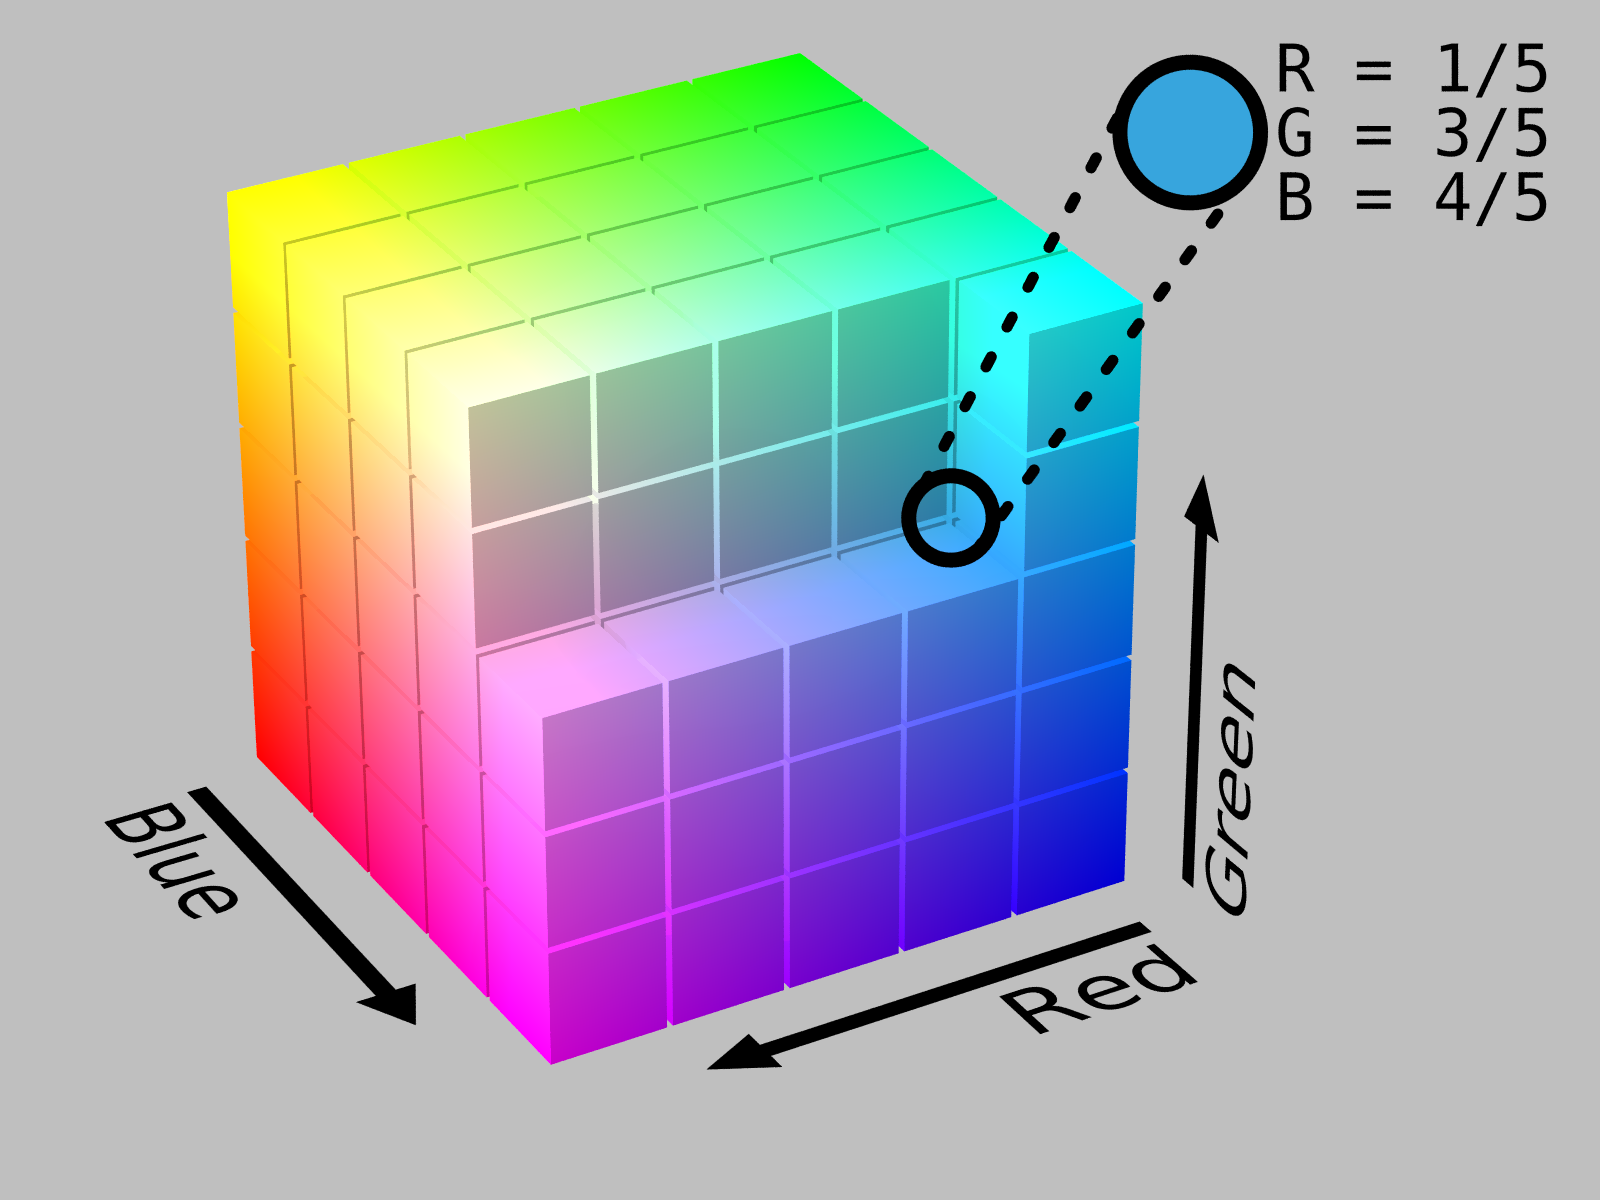
\includegraphics[scale=0.1]{RGBColorSpace}
\caption{RGB Color space}

\label{fig:RGBColorSpace}
\end{figure}

\subsection{HSV color space}\label{sec:PREPROC:hsv}

The HSV color space is one of the most common cylindrical-coordinate representations of points in an RGB color model. The hue is the human sensation according to which an area appears to be similar to one, or to proportions of two, of the perceived colors red, yellow, green and blue. The saturation is the colorfulness of an area relative to its brightness.  The value (brightness) is the human sensation by which an area exhibits more or less light. The color is then defined as a position on a circular plane around the value axes. Hue is the angle from a nominal point around the circle to the color while saturation is the radius from the central lightness axis to the color.

\begin{figure}[h]
\centering

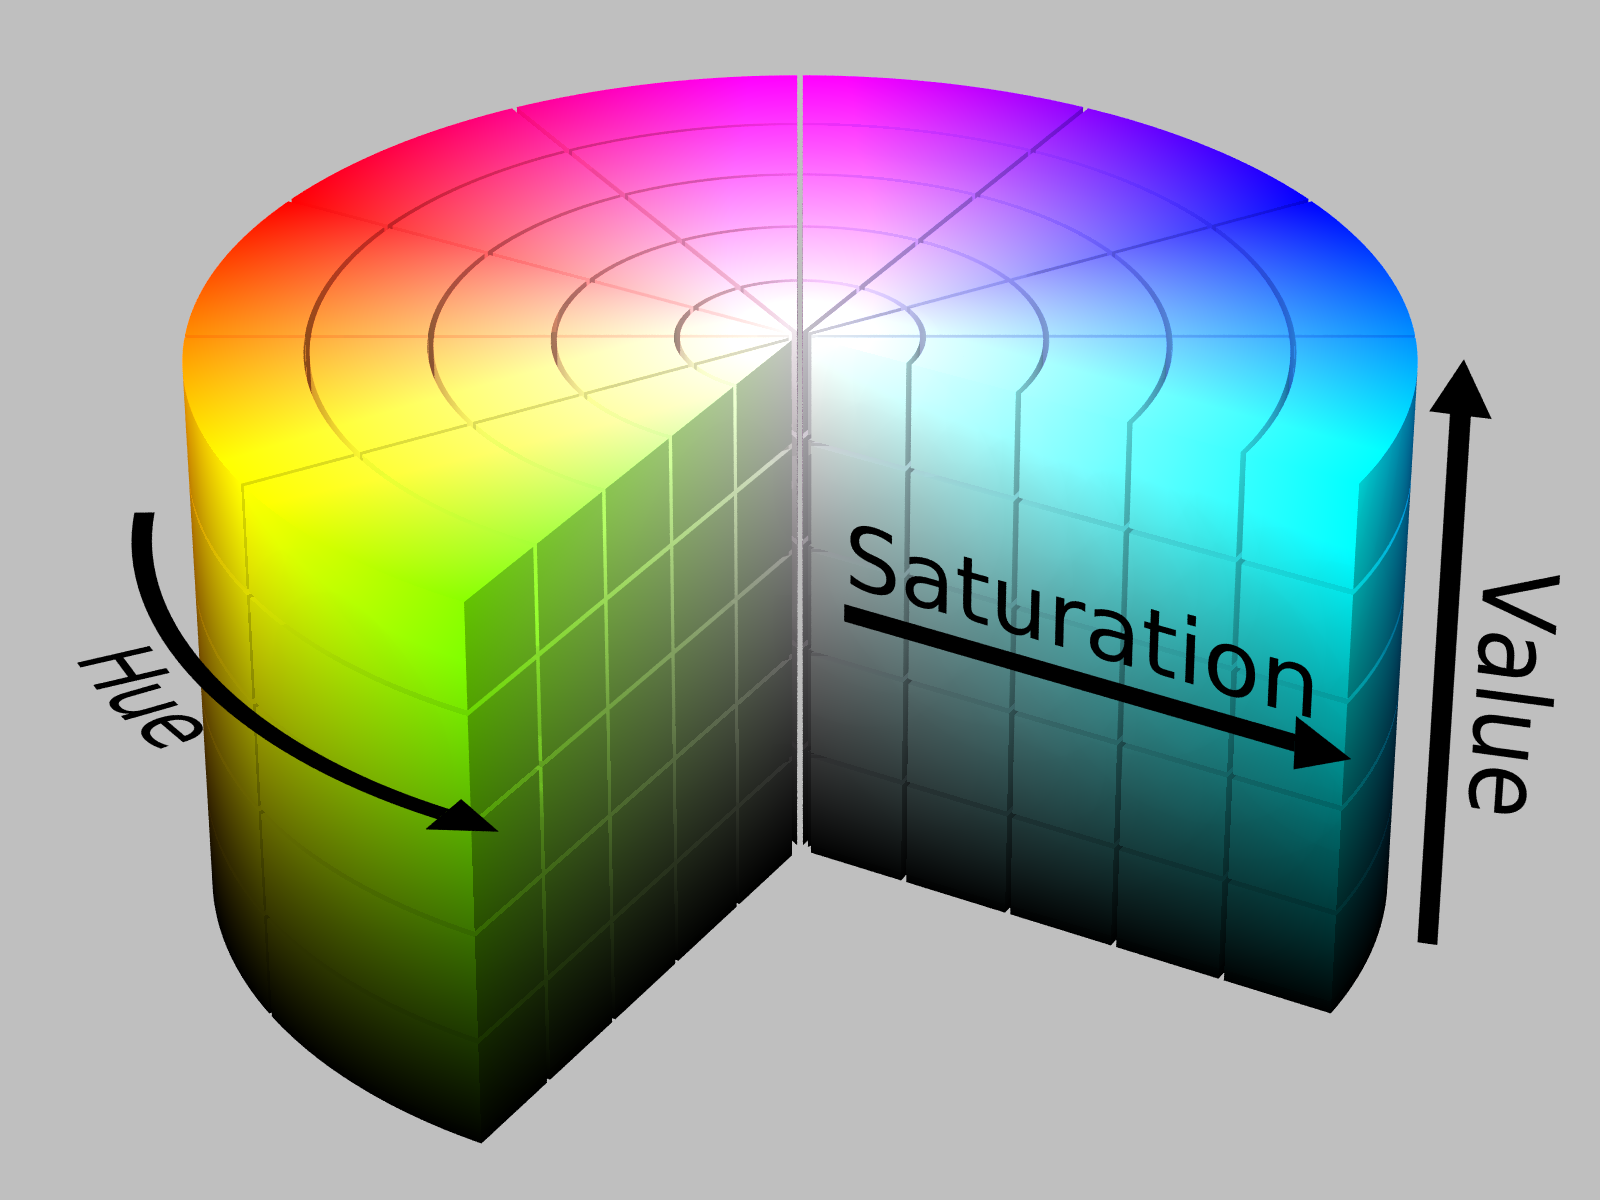
\includegraphics[scale=0.1]{HSVColorSpace}
\caption{HSV Color space}

\label{fig:HSVColorSpace}
\end{figure}

\section{Implementation}\label{sec:PREPROC:implement}



The traffic signs are meant to raise awareness therefore they use vivid colors, like red, yellow, blue, black, white. I create a new black and white image by filtering the colors of the original image. If the hue, saturation and value of a pixel satisfy a certain threshold, the pixel of the new image will be black otherwise white. I established these thresholds based on experiments and the \ref{fig:colorWheel} figure.

\begin{figure}[h]

\centering 
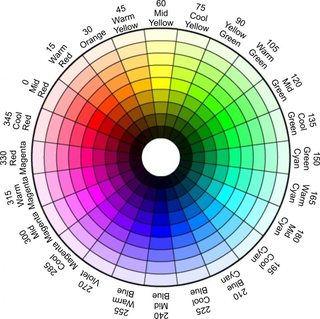
\includegraphics[scale=0.5]{ColorWheel}
\caption{Color wheel}
\label{fig:colorWheel} 

\end{figure}

%\begin{table}[H]
%\centering
%\begin{tabular}{ |p{3cm}||p{3cm}|p{3cm}|p{3cm}|  }
% \hline
% Country Name     or Area Name& ISO ALPHA 2 Code &ISO ALPHA 3 Code&ISO numeric Code\\
% \hline
% Afghanistan   & AF    &AFG&   004\\
% Aland Islands&   AX  & ALA   &248\\
% Albania &AL & ALB&  008\\
% Algeria    &DZ & DZA&  012\\
% American Samoa&   AS  & ASM&016\\
% Andorra& AD  & AND   &020\\
% Angola& AO  & AGO&024\\
% \hline
%\end{tabular}
%
%\caption{Table to test captions and labels}
%\label{table:1}
%\end{table}


%!TEX root = minta_dolgozat.tex
%%%%%%%%%%%%%%%%%%%%%%%%%%%%%%%%%%%%%%%%%%%%%%%%%%%%%%%%%%%%%%%%%%%%%%%
\chapter{Neurális hálók}\label{ch:INTRO}
%%%%%%%%%%%%%%%%%%%%%%%%%%%%%%%%%%%%%%%%%%%%%%%%%%%%%%%%%%%%%%%%%%%%%%%
\section{Bevezető}
\subsection{Biológiai modell}

Az idegsejtek (neuronok) az idegrendszer alkotóelemei. A neuron jeleket fogad és ezekre megfelelő választ generál. A \ref{fig:idegsejt} ábrán látható egy idegsejt és annak részei. A dendritek a bejövő információt szállítják, az idegrost egy szigetelt vezető, az axonvégek a választ szállítják tovább a velük kapcsolatban levő idegsejteknek. 

Az emberi idegrendszer nagyon komplex műveletek elvégzésére képes rövid idő alatt, ennek analógjára hozták létre a mesterséges neurális hálókat.

\begin{figure}[h]
\centering

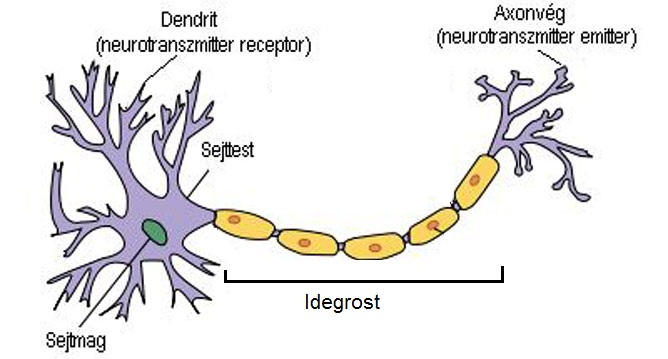
\includegraphics[scale=0.5]{images/idegsejt}
\caption{Idegsejt}

\label{fig:idegsejt}
\end{figure}


\section{Mesterséges neuronok}\label{sec:INTRO:neurons}
A neuronok a neurális hálók építőkövei.
\subsection{Szigmoid neuron}

A szigmoid neuron 0 és 1 közötti értékeket kap bementi paraméterként és létrehoz egy kimentet ugyanebben az intervallumban.

\begin{figure}[h]
\centering

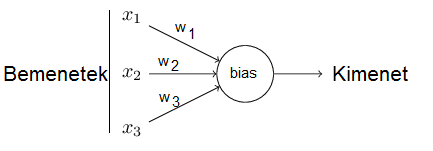
\includegraphics[scale=1]{images/neuron}
\caption{Sigmoid neuron}

\label{fig:neuron}
\end{figure}

Mindegyik bemenethez súlyok vannak rendelve, ami azt jelképezi, hogy az illető bemenet mennyire játszik fontos szerepet a neuron kimenetében. Minden neuronhoz tartozik továbbá egy "bias" ami a kisebb rendellenességek javítására szolgál.

A sigmoid neuron kimenete a \ref{eq:1} képlettel számítható ki.

\begin{equation} \label{eq:1}
\sigma(\sum\limits_{i=1}^{n-1} w_{i}*x_{i} + b)
\end{equation}

\begin{equation} \label{eq:2}
\sigma(z) = \frac{1}{1+e^{-z}}
\end{equation}

A \ref{eq:2} függvényt aktiválási függvénynek nevezik. Az aktiválási függvény szerepe, hogy a kimenetet egy adott intervallumba szorítsa. Ahogy ez a \ref{fig:sigmoidf} ábrán is látszik, a sigmoid neuron esetében ez az intervallum 0 és 1 között van. 

\begin{figure}[h]
\centering

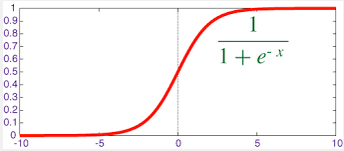
\includegraphics[scale=1]{images/sigmoidf}
\caption{Szigmoid függvény grafikus képe}

\label{fig:sigmoidf}
\end{figure}

A szigmoid neuron egyik tulajdonsága, hogy kis változás a súlyokban, kis változást eredményez a kimenetben. Ez legalább annyira előny is, mint hátrány. Előny, mert amikor a kimenet közel van az elvárt kimenethez, a módosítások nem eredményezik azt, hogy a kimenet túlságosan eltávolodjon az elvárttól. Hátrány, mert amikor a kimenet nagyon helytelen, mint például a tanulás elején, hosszú időbe telik a javítása.

\begin{figure}[h]
\centering

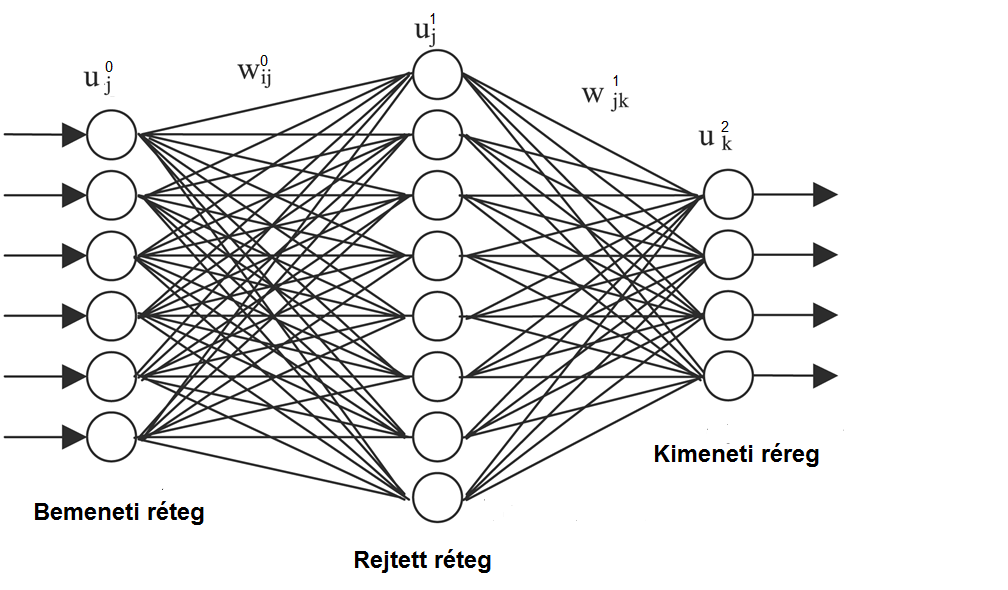
\includegraphics[scale=0.5]{images/net}
\caption{Egyszerű neurális háló}

\label{fig:net}
\end{figure}

A \ref{fig:net} ábrán egy egyszerű szigmoid neuronokból álló neurális háló látható. A súlyvektorok mérete már ennél a kis példánál is viszonylag nagy, ezért egy nagy hálónál ezek az értékek jelentősen megnőnek.


\section{Szerkezek}\label{sec:INTRO:architecture}

Olyan neurális hálót használtam, amelynek 625 bemenete és 43 kimenete van. A bemeneti neuronok a kép egy pixelének szürke árnyalatát tartalmazzák. A kimenetek száma megegyezik a forgalmi táblák osztályainak a számával. Különböző számú rejtett réteggel kísérleteztem, és ezeken belül is változó számú neuronnal.

\section{Sztochasztikus gradiens csökkentés}\label{sec:INTRO:graddesc}

Annak érdekében, hogy a súlyokat és bias-okat a kimenetnek az elvárt eredménytől való eltérése függvényében tudjam módosítani, a sztochasztikus gradiens csökkentést alkalmaztam. Ez a gradiens csökkentés egyszerűsített változata. Gradiens csökkentéssel a teljes tanítási adathalmazra számolja a hiba értékét, míg a sztochasztikus gradiens csökkentés közelíti a hibát egy bizonyos számú véletlenszerűen kiválasztott adat alapján. Minél nagyobb ez a szám, a közelítés pontossága annyival jobb lesz, de mivel nem a teljes adathalmazzal dolgozik, ezért gyorsabb lesz.

A \ref{eq:3} egyenlet a négyzetes hibafüggvény. \textit{n} a bemeneti tanítási adatok száma, \textit{y(x)} az \textit{x} bemenetre a háló által generált kimenet és \textit{a} az elvárt kimenet az \textit{x} bemenetre. Amikor az elvárt és a kiszámított kimenet közel van egymáshoz, a hiba kicsi lesz. Mivel a célom, hogy a kiszámított kimenet az elvárt kimenetet közelítse meg minél jobban, ezt a hibát kell minimalizálnom. Ennek érdekében bevezetem a  $\nabla C$-vel jelölt gradiensét a hibafüggvénynek. A gradiens értékét a \ref{eq:6} képlettel lehet kiszámítani.

\begin{equation} \label{eq:3}
\ C = \frac{1}{2n}\sum\nolimits_{x} \|y(x)-a(x)\|^2
\end{equation}

\begin{equation} \label{eq:6}
\ \nabla C = (\frac{\partial C}{\partial w_{i}},\frac{\partial C}{\partial b_{j}})^T
\end{equation}

A hiba csökkentése érdekében ismételtem alkalmaztam a \ref{eq:4} és a \ref{eq:5} szabályokat a súlyokra és bias-okra. $\eta$ a tanítási ráta. Ez egy kicsi érték kell legyen, de nem túl kicsi, mert akkor a tanulási folyamat túl lassú lenne.

\begin{equation} \label{eq:4}
\ w_{i} \rightarrow w_{i} - \eta\frac{\partial C}{\partial w_{i}} 
\end{equation}

\begin{equation} \label{eq:5}
\ b_{j} \rightarrow b_{j} - \eta\frac{\partial C}{\partial b_{j}} 
\end{equation}


\section{Backpropagation}\label{sec:INTRO:backprop}


A backpropagation algoritmus arra szolgál, hogy a háló súlyait és bias-ait úgy állítsa be, hogy a kimenet megközelítse minél jobban az elvárt kimenetet.

A \ref{eq:7} egyenletben $z^l$ a súlyozott bementi vektor az l-edik rétegben. Ahogy a \ref{eq:8} egyenletben látható, a kimeneti vektor egy rétegben az előző réteg kimenetének használatával számolható ki, vagyis az információ továbbításával. A háló kimenetének kiszámítása után a \ref{eq:9}-es egyenlet segítségével lehet kiszámolni az utolsó réteg hibáját, ahol \textit{L} a rétegek számát jelöli, \textit{$\nabla_aC$} pedig a $\frac{\partial C}{\partial a_j^L}$ parciális deriváltakat tartalmazó vektor.


Maga a backpropagation a \ref{eq:10} képlet segítségével történik minden \textit{l} rétegre, \textit{L-1}-től 2-ig.

\begin{equation} \label{eq:7}
\ z^l = (w^l*a^{l-1} + b^l) 
\end{equation}

\begin{equation} \label{eq:8}
\ a^l = \sigma(z^l) 
\end{equation}

\begin{equation} \label{eq:9}
\ \delta^L = \nabla_aC \circ \sigma'(z^L)
\end{equation}

\begin{equation} \label{eq:10}
\ \delta^l = ((w^{l+1})^T* \delta^{l+1}) \circ \sigma'(z^l)
\end{equation}

\chapter{Az algoritmus} \label{algorihm}

\begin{enumerate}
   \item Súlyok és bias-ok inicializálása véletlenszerű adatokkal
   \item Minden ciklusra végezd:
   \begin{enumerate}
   		\item Tanulási adatok összekeverése
   		\item Minden batch-re végezd:
   		\begin{enumerate}  %updateMinibatch
   			\item Minden tanulási adatra a batch-ből végezd:
			    \begin{enumerate}
			      \item Mindegyik neuron kimenetének a kiszámítása a bemenettől a kimenet felé
			      \item Kimenet hibájának kiszámítása
		    	  \item Minden neuron hibájának kiszámítása a kimenettől a bemenet felé haladva
			    \end{enumerate}
		    \item Gradiens csökkentés: súlyok és bias-ok újraszámolása 
   		\end{enumerate}
   \end{enumerate}
   
 \end{enumerate}
 
 Ahhoz, hogy a háló tanulni tudjon, fontos az, hogy a súlyokat és bias-okat megfelelően kicsi számokkal inicializáljuk. Ezt úgy valósítottam meg, hogy a 0 és 1 között véletlenszerűen generált számot elosztottam 3000-el.
 
 A batch-ben egyidőben jelen levő adatok minél változatosabbak kell legyenek, annak érdekében hogy tanulás közben egy időben figyelembe vegye a különböző osztályok tulajdonságait. Ezért van szükség az adatok összekeverésére. A beolvasás sorban történik, vagyis az azonos osztályba tartozóak egymás után fognak szerepelni. Ha ebben a sorrendben kerülnének be a batch-be, akkor a háló először megpróbálná megtanulni az egyik osztály tulajdonságait, utána pedig sorban a következőkét. Az adatok keverésével ezt kerülöm el. \cite{5}

{

\bibliography{konyveszet}
\bibliographystyle{ieeetr}
}


\end{document}
